\section{Resultados}
En esta sección se muestran las secciones transversales para elipsoides oblatos, empleados como una primera aproximación a la forma discoide cóncava de los eritrocitos. Dado que los eritrocitos en una muestra real no interactúan fuertemente entre ellos \footnote{El contraste en el índice de refracción entre los eritrocitos y el plasma sanguíneo es relativamente bajo (0.04 - 0.06) \cite{RefracIndBlood}.} y que se encuentran orientados de forma aleatoria, es posible estudiar su respuesta óptica considerando una sola partícula y definir una respuesta promedio en términos de las secciones transversales promedio $\langle C_{ext} \rangle$, $\langle C_{abs} \rangle$ y $\langle C_{sca} \rangle$. Con estas cantidades, se considera que una onda plana puede excitar de forma eficiente el sistema en sus tres ejes de forma homogénea. \footnote{Considerando que las partículas no sean ópticamente activas.} Estas están dadas por \cite{Bohren}:
\begin{align*}
	\langle C_{abs}\rangle &= \frac{k}{3} \text{Im}\{\alpha^{(1)}+\alpha^{(2)}+\alpha^{(3)}\},\\
	\langle C_{sca}\rangle &= \frac{k^4}{3(6\pi)} \left(\alpha^{(1)}+\alpha^{(2)}+\alpha^{(3)}\right)^2.
\end{align*}

Para caracterizar la respuesta dieléctrica del material, se emplea la función dieléctrica $\epsilon(\omega)$, la cual puede determinarse experimentalmente a partir del índice de refracción complejo de un medio, $\tilde{n}(\omega) = n(\omega) + i\kappa(\omega)$. La relación entre la función dieléctrica y el índice de refracción está dada por las expresiones \cite{Plasmonics}
\begin{align} 
	\text{Re}[\epsilon(\omega)] &= n^2 - \kappa^2,\\
	\text{Im}[\epsilon(\omega)] &= 2n\kappa, \end{align}
donde $\kappa$ es el coeficiente de extinción, el cual describe la absorción de las ondas electromagnéticas al propagarse en el medio \cite{Plasmonics}.\\

Debido a su dependencia exclusiva de la frecuencia, es conveniente expresar a la función dieléctrica mediante el modelo de Drude, pues ofrece un mayor control sobre la respuesta óptica del sistema, resultando adecuado para estudiar la respuesta general y familiarizarse con el problema. El modelo de Drude es particularmente útil para describir el comportamiento plasmónico de materiales a energías bajas y en los que la respuesta óptica está dominada por electrones libres, como en los metales, donde los electrones en la banda de conducción responden colectivamente a un campo electromagnético aplicado. Mediante este modelo, se expresa a la función dieléctrica como \cite{Plasmonics}
\begin{equation} \epsilon(\omega) = 1 - \frac{\omega_p^2}{\omega^2 + i\gamma\omega}, \end{equation}
donde $\omega_p$ es la frecuencia de plasma del material y $\gamma$ es la constante fenomenológica de amortiguamiento. \\

Para analizar las contribuciones de las secciones transversales en partículas elipsoidales oblatas dentro del régimen cuasiestático, en la Fig. \ref{Contribuciones} se muestran las $\langle C_{abs} \rangle$ (línea roja) y $\langle C_{sca} \rangle$(línea verde). Estas cantidades se grafican en escala logarítmica en función de la longitud de onda $\lambda$ (eje superior) y la energía $\hbar\omega$ (eje inferior) de la onda electromagnética incidente. Las partículas se modelan utilizando una función dieléctrica descrita por el modelo Drude, con parámetros son $\hbar\omega_p=13.142\text{ eV}$ y $\hbar\gamma=0.197\text{ eV}$. Los semiejes de las partículas son $a=1.5\text{ nm}$, $c=1\text{ nm}$. Además, las están inmersas en una matriz con un índice de refracción de $n_m=1.33$. \\
\begin{figure}[h!]
	\sidesubfloat[]{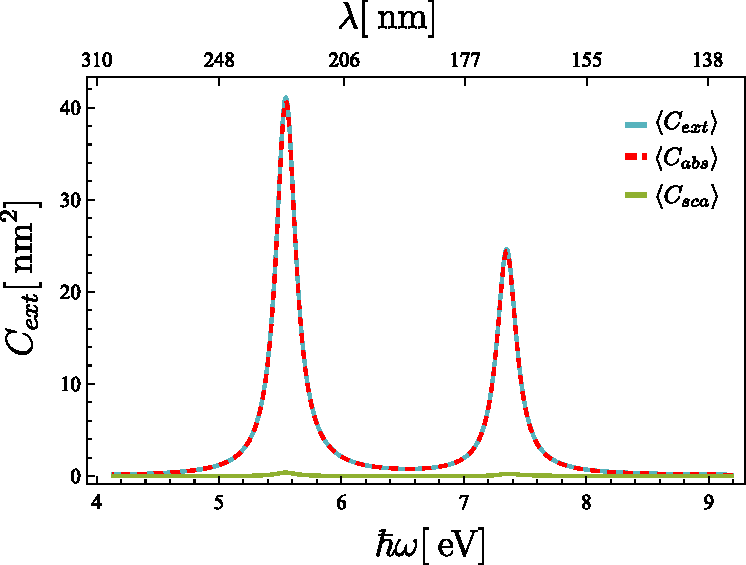
\includegraphics[width=.445\textwidth]{../../Figuras/AlContribuciones3.pdf} \label{Contribuciones}}\quad%
	\sidesubfloat[]{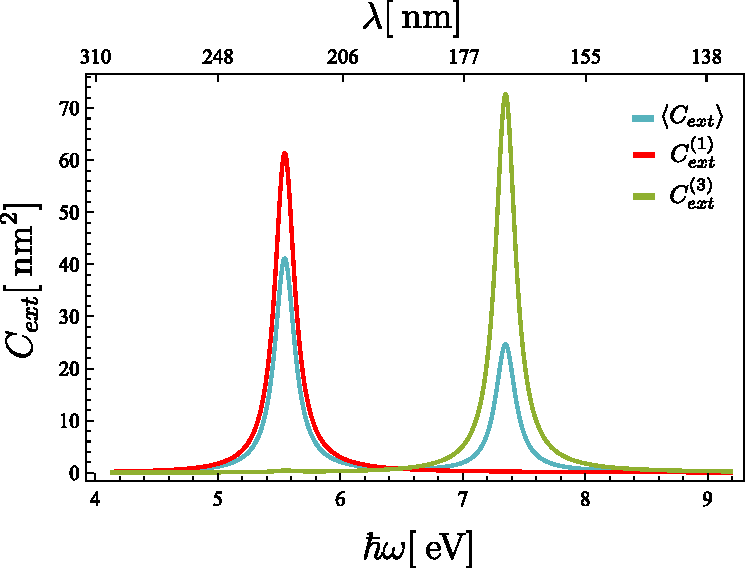
\includegraphics[width=.44\textwidth]{../../Figuras/CextAlbueno.pdf}\label{Cextpromedio}}%
	\caption{Secciones transversales como función de la energía $\hbar\omega$ (eje inferior) y de la longitud de onda $\lambda$ (eje superior) para una partícula elipsoidal oblata de aluminio caracterizada por su función dieléctrica dada por el modelo de Drude ($\hbar\omega_p=13.142\text{ eV}$, $\hbar\gamma=0.197\text{ eV}$), con semiejes $a=b=1.5\text{ nm}$, $c=1\text{ nm}$ e inmersa en un medio acuoso ($n_m=1.33$). \textbf{a)}  Sección transversal de extinción promedio $\langle C_{ext}\rangle$  (línea azul), sección transversal de absorción promedio $\langle C_{abs}\rangle$  (línea roja) y sección transversal de esparcimiento promedio $\langle C_{sca}\rangle$  (línea verde) en escala logarítmica. \textbf{b)} Sección transversal de extinción promedio $\langle C_{ext}\rangle$ (línea azul), sección transversal de extinción al iluminar a la partícula con una onda polarizada en la dirección $\hat{e}_x$, $C_{ext}^{(1)}$  (línea roja)  y sección transversal de extinción al iluminar la partícula con una onda polarizada en la dirección $\hat{e}_z$ $C_{ext}^{(3)}$  (línea verde).} \label{fig:test}
\end{figure}

A partir de los resultados mostrados en la Fig. \ref{Contribuciones}, se observa que, en partículas dentro del régimen cuasiestático, la absorción domina sobre el esparcimiento en la contribución a la extinción. Esto se evidencia en la diferencia de magnitudes entre ambas curvas, donde la absorción es aproximadamente tres órdenes de magnitud mayor que el esparcimiento y la curva de extinción es escencialmente la misma que la de absorción. Debido a esta marcada diferencia, los análisis posteriores se enfocan exclusivamente en las secciones transversales de extinción, ya que la contribución del esparcimiento es despreciable.\\

El análisis de las diferencias entre la $\langle C_{ext}\rangle$ y  las secciones transversales de extinción obtenidas al iluminar la partícula con una onda polarizada en una única dirección, se presenta en la Fig. \ref{Cextpromedio}. En esta figura se muestra la $\langle C_{ext}\rangle$ (línea azul), $C_{ext}^{(1)}$ (línea roja) y $C_{ext}^{(3)}$ (línea verde) en función de $\lambda$ (eje superior) y $\hbar\omega$ (eje inferior) de la onda electromagnética incidente. Estos cálculos corresponden a un sistema con las mismas características que el de la Fig. \ref{Contribuciones}.\\

En la Fig. \ref{Cextpromedio} se observa que debido a la geometría de la partícula, que es un elipsoide oblato, la 
$\langle C_{ext}\rangle$ presenta dos máximos, los cuales coinciden con las frecuencias de los máximos de $C_{ext}^{(1)}$ y $C_{ext}^{(3)}$. Esto muestra que las secciones transversales promedio son útiles para representar el efecto de iluminar una partícula elipsoidal con una onda electromagnética polarizada en la dirección de cualquiera de sus tres ejes principales, ya que lo que cambia es el valor nominal de los máximos en la sección transversal promedio, más no la localización espectral de estos. \\

Las siguientes figuras presentan los cálculos de las secciones tranversales de extinción promedio  $\langle C_{ext}\rangle$ considerando nanopartículas elipsoidales oblatas cuya función dieléctrica está caracterizada por el modelo de Drude para aluminio \cite{Aluminio} y por datos experimentales para plata \cite{Plata}, oro \cite{Plata}, bismuto \cite{Bismuto} y  óxido de magnesio \cite{MgO}.


\subsection*{Aluminio y plata}
En la Fig. \ref{aluminioplataAR} se muestran las $\langle C_{ext}\rangle$ en función de $\hbar\omega$ (eje inferior) y de  $\lambda$ (eje superior) de la onda electromagnética incidente en nanopartículas elipsoidales oblatas de aluminio (AlNPs) (Fig. \ref{aluminioAR}) y plata (AgNPs) (Fig.~\ref{plataAR}). La función dieléctrica para las AgNPs está dada por el modelo de Drude con parámetros $\hbar\omega_p=13.142\text{ eV}$, $\hbar\gamma=0.197\text{ eV}$, mientras que para las AlNPs  está dada por datos experimentales obtenidos de \cite{Plata}. Se realizan los cálculos para partículas elipsoidales con razón de aspecto AR=2 y con semiejes de tamaños desde 1 nm a 2.5 nm, en pasos de 0.5 nm; cada caso se identifica con el código de color mostrado en la gráfica. Además, se incluye los cálculos para una partícula esférica con $a=2 \text{ nm}$ y (línea gris punteada) con relación de aspecto AR$=1$. Todas las partículas se consideran inmersas en un medio acuoso con $n_m=1.33$.\\

\begin{figure}[h!]
	\sidesubfloat[]{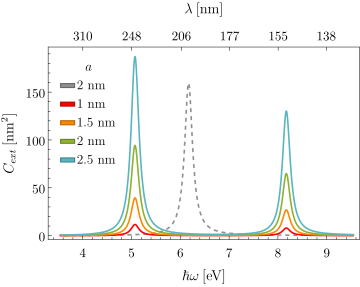
\includegraphics[width=.445\textwidth]{../../Figuras/AlAR} \label{aluminioAR}}\quad%
	\sidesubfloat[]{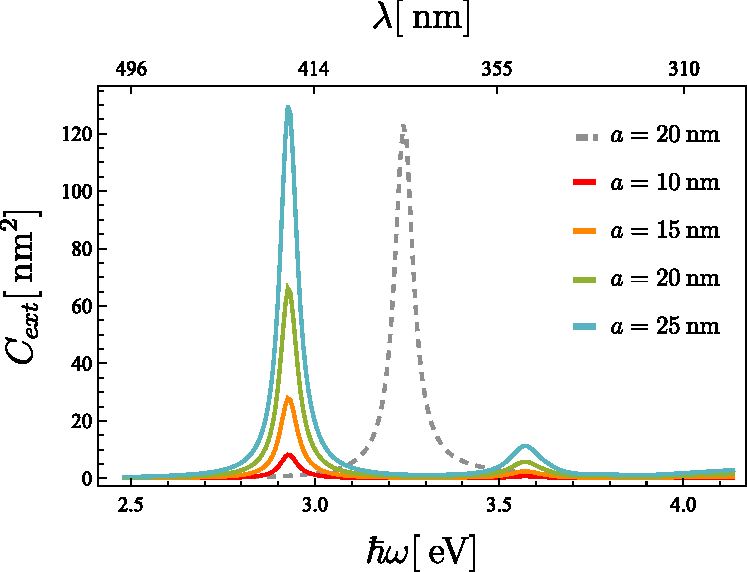
\includegraphics[width=.44\textwidth]{../../Figuras/AgAR}\label{plataAR}}%
	\caption{Secciones transversales de extinción promedio como función de la energía (eje inferior) y de la longitud de onda (eje superior) de la onda electromagnética incidente para una partícula elipsoidal oblata inmersa en un medio acuoso ($n_m=1.33$). Las partículas poseen AR=2, excepto en el caso de la línea gris punteada en el que AR=1 (partícula esférica). Además, están caracterizadas por su función dieléctrica dada por  \textbf{a)} el modelo de Drude para el aluminio con parámetros $\hbar\omega_p=13.142\text{ eV}$ y $\hbar\gamma=0.197\text{ eV}$) y \textbf{b)} datos experimentales correspondientes a la plata obtenidos de \cite{Plata}. }\label{aluminioplataAR}
\end{figure}
A partir de los resultados de la Fig. \ref{aluminioplataAR}, se observa que al aumentar el tamaño de la partícula mientras se mantiene constante AR, la localización espectral de las resonancias no cambia pero su valor nominal aumenta. Se identifican dos máximos locales en $\langle C_{ext}\rangle$,  los cuales corresponden a las frecuencias en las que $C_{ext}^{(1)}$ y $C_{ext}^{(3)}$ se maximizan. Para $C_{ext}^{(1)}$, las resonancias  se encuentran en $\lambda=$254 nm (4.88 eV) para las AlNPs y $\lambda=$434 nm (2.86 eV) para las AgNPs. Para $C_{ext}^{(3)}$, las resonancias ocurren en $\lambda=$146 nm (8.5 eV) para AlNPs y $\lambda=$344 nm (3.6 eV) para las AgNPs. \\

El efecto de la variación de la razón de aspecto en la sección transversal de extinción promedio en AlNPs y AgNPs inmersas en un medio acuoso con $n_m=1.33$ se muestra en la Fig. \ref{aluminioplatac}. En esta figura, las partículas elipsoidales se consideran con AR entre 1.5 a 2.25, con incrementos 0.25 y con un semieje menor fijo de $c=1\text{ nm}$ y también se incluye $\langle C_{ext}\rangle$ para una partícula esférica con  $c=1\text{ nm}$ y con razón de aspecto AR$=1$. Las funciones dieléctricas empleadas son las mismas que en la Fig. \ref{aluminioplataAR}.


\begin{figure}[h!]
	\sidesubfloat[]{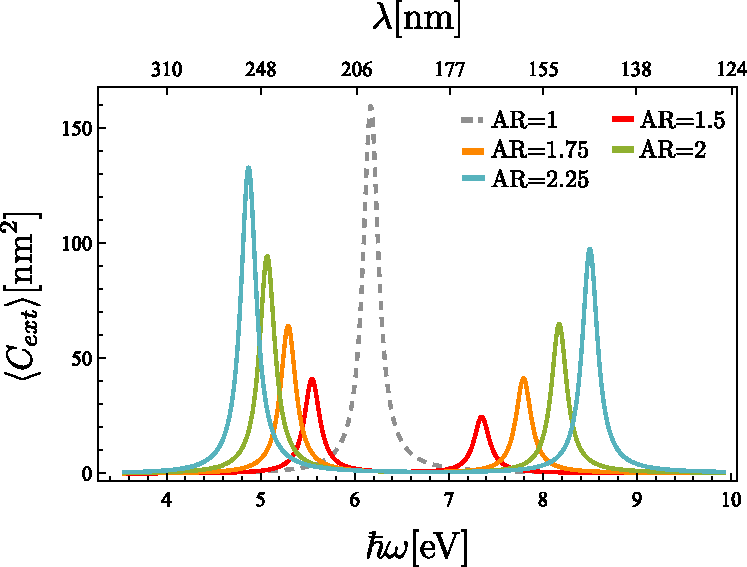
\includegraphics[width=.445\textwidth]{../../Figuras/Alc} \label{aluminioc}}\quad%
	\sidesubfloat[]{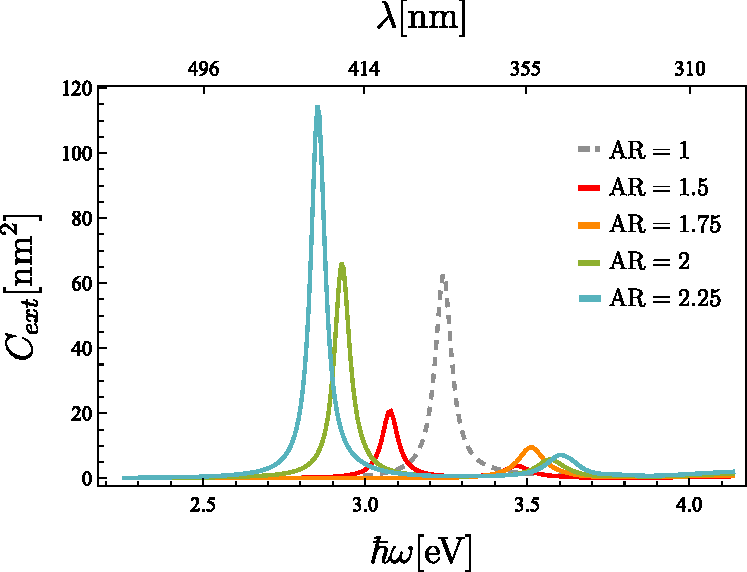
\includegraphics[width=.44\textwidth]{../../Figuras/Agc}\label{platac}}%
	\caption{Secciones transversales de extinción promedio como función de la energía (eje inferior) y de la longitud de onda (eje superior) de la onda electromagnética incidente para una partícula elipsoidal oblata inmersa en un medio acuoso ($n_m=1.33$). Las partículas  poseen un semieje menor de tamaño $c=1nm$ y presentan diferentes AR cuyo código de color se observa en la gráfica. Además, están inmersas en un medio acuoso ($n_m=1.33$) y están caracterizadas por su función dieléctrica dada por  \textbf{a)} el modelo de Drude para el aluminio ($\hbar\omega_p=13.142\text{ eV}$, $\hbar\gamma=0.197\text{ eV}$) y \textbf{b)} datos experimentales correspondientes a la plata obtenidos de \cite{Plata}.}\label{aluminioplatac}
\end{figure} 

 En las Figs. \ref{aluminioc}  y \ref{platac} se observa que conforme la relación de aspecto se aproxima a la unidad, hay un corrimiento de las frecuencias asociadas a las $\langle C_{ext}\rangle$ máximas hacia la frecuencia de resonancia asociada a una partícula esférica. Esta frecuencia de resonancia corresponde a $\lambda=201\text{ nm}$ (6.17 eV) para el aluminio y $\lambda=383\text{ nm}$ (3.24 eV) para la plata. Además, tanto en el aluminio como en la plata, se observa que al aumentar la relación de aspecto y la longitud del eje mayor, el valor nominal de  $\langle C_{ext}\rangle$ también aumenta. Esto se debe a que una mayor sección transversal efectiva de interacción con la onda electromagnética incrementa la probabilidad de esparcimiento y absorción de luz, lo que, en consecuencia, aumenta la extinción.



\subsection*{Oro y bismuto}
De forma análoga al análisis en la variación de los parámetros geométricos de las AlNPs y AgNPs, se muestra en la Fig. \ref{oro} la respuesta óptica variando estos parámetros (semieje mayor y razón de aspecto) considerando ahora una función dieléctrica de un material real. En particular, en Fig. \ref{oroAR} se grafica $\langle C_{ext}\rangle$ como función de $\hbar\omega$ (eje inferior) y de $\lambda$ (eje superior) para nanopartículas elipsoidales oblatas de oro (AuNPs) de distintos tamaños que conservan la razón de aspecto de AR=2; para complementar el análisis, se muestra debajo de esta gráfica la función dieléctrica del oro donde los puntos representan los datos obtenidos de \cite{Plata} y las líneas continuas corresponden a una interpolación. En la Fig. \ref{oroAR} se consideran partículas con relación de aspecto AR$=2$ con radios desde 1  nm a 2.5 nm, con incrementos de 0.5 nm; cada caso se identifica con el código de color mostrado en la gráfica respectiva. También se considera una partícula con relación de aspecto AR$=1$ y semiejes $a=2$ nm (línea gris punteada), que representa a una partícula esférica. Por otro lado, en la Fig. \ref{oroc} se consideraron partículas con relación de aspecto variable AR=1.5 (línea roja), AR=1.75 (línea naranja), AR=2 (línea verde) y AR=2.25 (línea azul) que presentan valores en su semieje menor $c=1\text{ nm}$. Asimismo, se considera una partícula esférica con semieje mejor $c=1\text{ nm}$ y con relación de aspecto AR$=1$ (línea gris).
\begin{figure}[H]
	\sidesubfloat[]{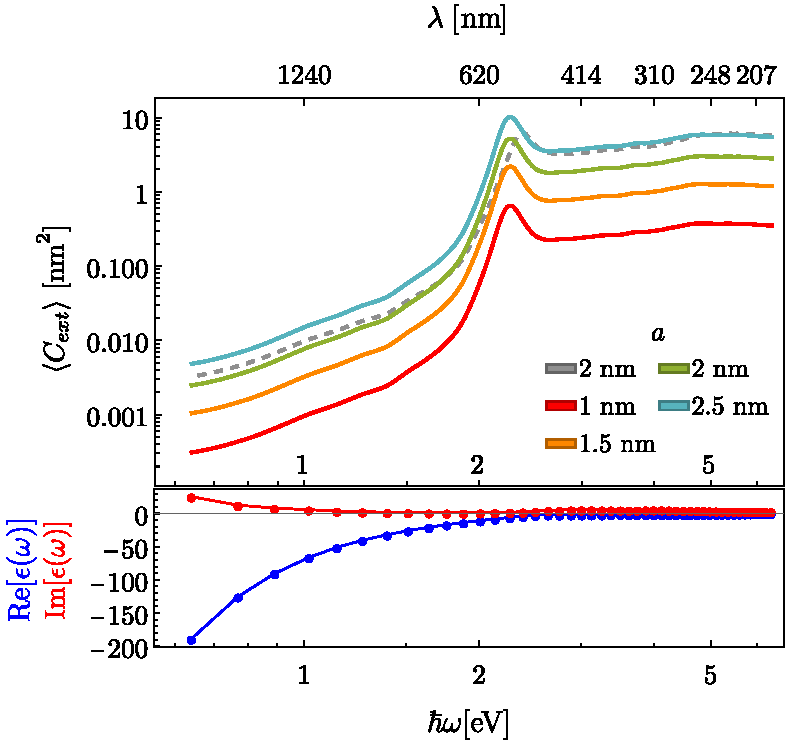
\includegraphics[width=.445\textwidth]{../../Figuras/Au2.pdf} \label{oroAR}}\quad%
	\sidesubfloat[]{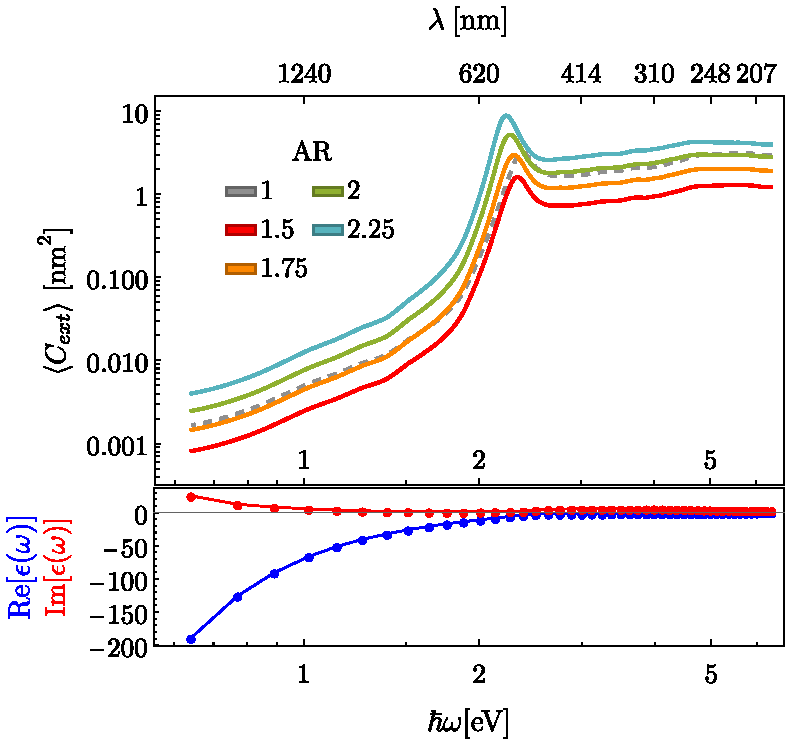
\includegraphics[width=.44\textwidth]{../../Figuras/Au.pdf}\label{oroc}}%
	\caption{Secciones transversales de extinción promedio como función de la energía (eje inferior) y de la longitud de onda (eje superior) para una partícula elipsoidal oblata de oro inmersa en un medio acuoso con $n_m=1.33$, y cuyo índice de refracción complejo fue obtenido a partir de datos experimentales de \cite{Plata}. Debajo de las gráficas se muestra la función dieléctrica del oro obtenida a partir de \cite{Plata} (parte real en azul, parte imaginaria en rojo). La línea recta que une los puntos experimentales fue obtenida mediante una interpolación. \textbf{a)} AuNPs con AR=2, excepto en el caso de una esfera (línea gris punteada) donde AR=1. \textbf{b)} AuNPs con semieje menor $c=1$ nm.}\label{oro}
\end{figure}

En contraste con el aluminio y la plata, para el oro se observa solo una excitación plasmónica en $\lambda=$ 547 nm (2.27 eV). Esta excitación se encuentra a la izquierda de la de la esfera en $\lambda=$ 557 nm (2.23 eV) y se esperaría que existiera otra a la izquiera de esta, como en los casos anteriores. Esto se atribuye a la fuerte absorción del oro a energías altas, lo que suprime resonancias atribuidas a contribuciones no descritas por el modelos de Drude en los datos experimentales. \footnote{En particular de contribuciones dieléctricas descritas por el modelo de Lorentz \cite{Plasmonics}.} Por otro lado, un resultado que sigue las tendencias observadas en las AlNPs y AgNPs que se observa en las AuNPs es la consistencia en la AR que reproduce el caso de una esfera en su respuesta espectral cuando AR tiende a la unidad. \\

En los casos anteriores se analizó el aluminio, que es bien descrito por el modelo de Drude y metales nobles como la plata y el oro. Ahora, en la Fig. \ref{bismuto} se muestran las secciones transversales de extinción promedio en función de la energía (eje inferior) y la longitud de onda (eje superior) para nanopartículas elipsoidales oblatas de bismuto (BiNPs), un semimetal. Como complemento, debajo de las gráficas se muestra la función dieléctrica del bismuto obtenida de \cite{Bismuto}. En la Fig. \ref{bismutoAR} se consideraron partículas con  AR$=2$  y en la Fig. \ref{bismutoc} se consideraron partículas con relación de aspecto variable desde 1.5 hasta 2.25, con incrementos de 0.25. 

\begin{figure}[H]
	\sidesubfloat[]{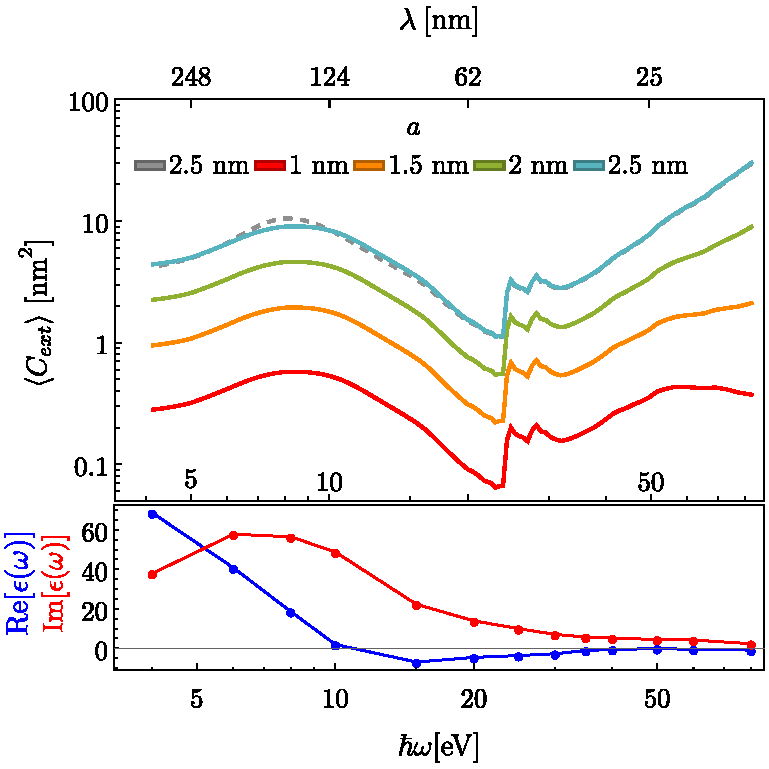
\includegraphics[width=.445\textwidth]{../../Figuras/Bi2} \label{bismutoAR}}\quad%
	\sidesubfloat[]{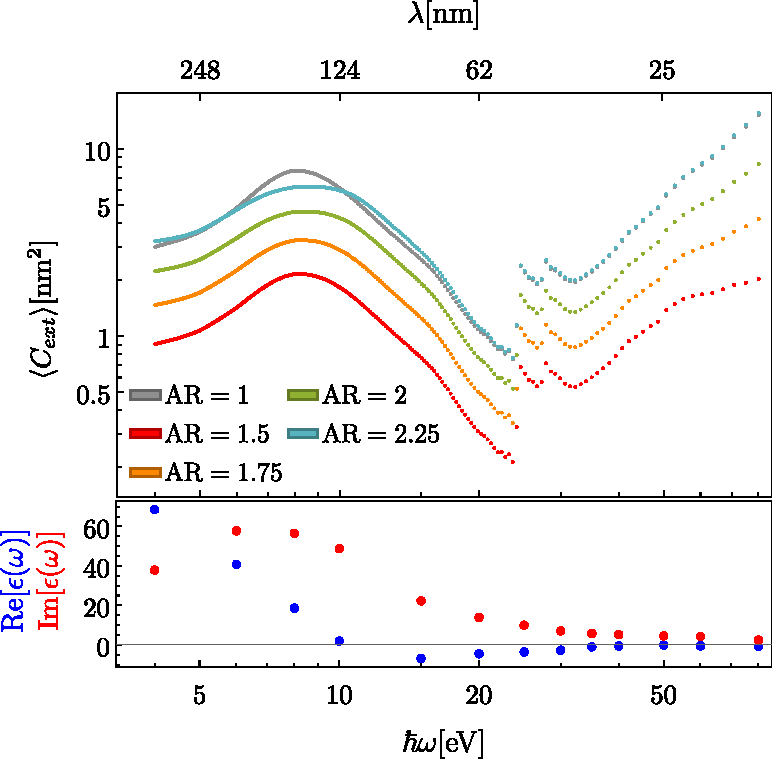
\includegraphics[width=.44\textwidth]{../../Figuras/Bi}\label{bismutoc}}%
	\caption{Secciones transversales de extinción promedio  como función de la energía (eje inferior) y de la longitud de onda (eje superior) para una partícula elipsoidal oblata de bismuto inmersa en un medio acuoso con $n_m=1.33$, y cuyo índice de refracción complejo fue obtenido a partir de datos experimentales de \cite{Bismuto}. Debajo de las gráficas se muestra la función dieléctrica del oro obtenida a partir de \cite{Plata} (parte real en azul, parte imaginaria en rojo). La línea recta que une los puntos experimentales fue obtenida mediante una interpolación. \textbf{a)} BiNPs con AR=2, excepto en el caso de una esfera (línea gris punteada) donde AR=1. \textbf{b)} BiNPs con semieje menor $c=1$ nm.}\label{bismuto}
\end{figure}

En ambas figuras se observan frecuencias de resonancia alrededor de $\lambda=147$ nm (8.44 eV), que se encuentran a la izquierda de la frecuencia de resonancia en $\lambda=154$ nm (8.03 eV) correspondiente a una nanopartícula esférica y de manera similar al caso del oro, se esperaría que existiera otra resonancia a la izquierda de la de la esfera. También se observa un aumento de la $\langle C_{ext}\rangle$ a partir de $\lambda=50$ nm  que se atribuye a contribuciones no descritas por el modelo de Drude en los datos experimentales. Como en los casos anteriores, se observa que al aproximar AR a la unidad, se recupera la frecuencia de resonancia correspondiente a una nanopartícula esférica.



\subsection*{Óxido de magnesio}
Finalmente, las $\langle C_{ext}\rangle$ para un material dieléctrico: el óxido de magnesio (MgO) se muestran en la Fig. \ref{mgo}. En esta gráfica se realiza la variación de la AR y el semieje mayor en nanopartículas elipsoidales oblatas de óxido de magnesio (MgONPs). Las $\langle C_{ext}\rangle$ se grafican en función de la energía (eje inferior) y de la longitud de onda (eje superior). De la misma forma que con los materiales anteriores, se consideraron partículas con relación de aspecto AR$=2$ con radios desde 1  nm a 2.5 nm, con incrementos de 0.5 nm, con su respectivo código de color indicado en la gráfica (Fig. \ref{mgoAR}) y en la Fig. \ref{mgoc} se consideraron partículas con AR variable. 

\begin{figure}[H]
	\sidesubfloat[]{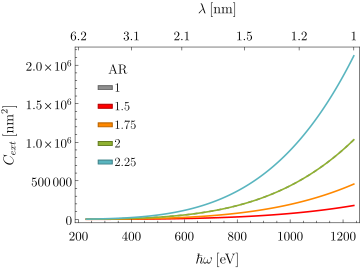
\includegraphics[width=.445\textwidth]{../../Figuras/MgOc} \label{mgoc}}\quad%
	\sidesubfloat[]{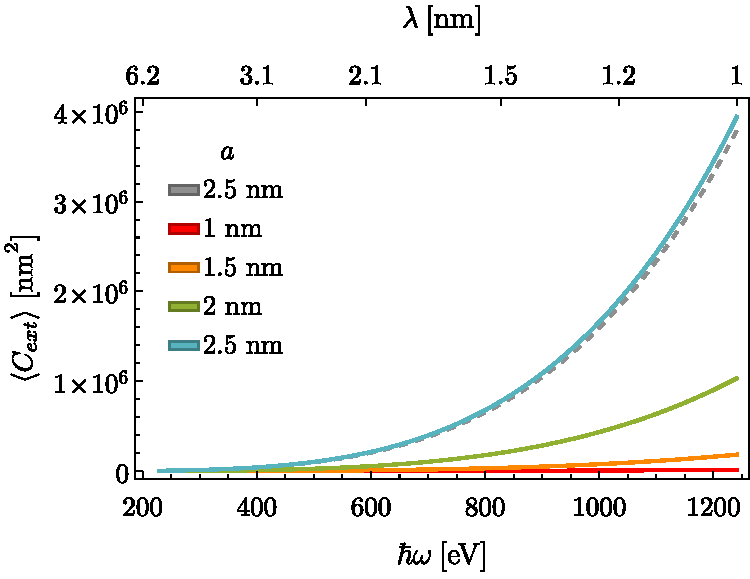
\includegraphics[width=.44\textwidth]{../../Figuras/MgOAR}\label{mgoAR}}%
	\caption{Secciones transversales de extinción promedio como función de la energía (eje inferior) y de la longitud de onda (eje superior) para una partícula elipsoidal oblata de óxido de magnesio inmersa en un medio acuoso ($n_m=1.33$). \textbf{a)} MgONPs con AR=2, excepto en el caso de una esfera (línea gris punteada) donde AR=1. \textbf{b)}  MgONPs con semieje menor $c=1$ nm.}\label{mgo}
\end{figure}

En ambos casos se observa que la $\langle C_{ext}\rangle$ tiene un comportamiento creciente y no se observan resonancias plasmónicas debido a la naturalez dieléctrica del óxido de magnesio. Esto también se atribuye a que en el rango de energías analizado existen procesos de absorción no descritos por el modelo de Drude.








